\documentclass[t]{beamer}

% Load general definitions
% Preamble file - general definitions, package loading, etc.

%=================================
% Load packages
\usepackage{amssymb,amsmath}
\usepackage{graphicx}
\usepackage{url}
\usepackage{tikz}
\usetikzlibrary{mindmap,trees,arrows}
\usepackage{fancyvrb}
\usepackage[portuguese]{babel} 
\usepackage[utf8]{inputenc}
\usepackage{subfigure}
\usepackage{times}
\usepackage[T1]{fontenc}
\usepackage{cancel}
\usepackage{color}
\usepackage{listings}
\usepackage[document]{ragged2e}
\usepackage{hyperref}
\usepackage{listings}


%=================================
% Set mode
\mode<presentation>
{
	\usetheme{Madrid}
	\usecolortheme{structure}
	\useoutertheme{infolines}
	\setbeamercovered{invisible}
}

% Get rid of nav bar
\beamertemplatenavigationsymbolsempty

% Insert frame number at bottom of the page.
\usefoottemplate{\hfil\tiny{\color{black!90}\insertframenumber}} 

%=================================
% Define new commands

\newcommand\Real{{\mathbb{R}}}
%\newcommand{\vi}{\vspace{0.6\baselineskip}}
%\newcommand{\goodgap}{\hspace{\subfigtopskip}\hspace{\subfigbottomskip}}


% Equation environments
\newcommand{\beq}{\begin{equation}}
\newcommand{\eq}{\end{equation}}
\newcommand{\beqs}{\begin{equation*}}
\newcommand{\eqs}{\end{equation*}}
\newcommand{\beqn}{\begin{eqnarray}}
\newcommand{\eqn}{\end{eqnarray}}
% Bold variables
\newcommand{\mbf}[1]{\ensuremath{\mathbf{#1}}}
% Itemization
\newcommand{\bitem}{\begin{itemize}}
\newcommand{\eitem}{\end{itemize}}
\newcommand{\spitem}{\vskip 1em\item}
\newcommand{\bitems}{\begin{itemize}\item}
\newcommand{\benums}{\begin{enumerate}\item}
\newcommand{\eenum}{\end{enumerate}}
% color blocks
\newenvironment{colorblock}[2]{%
\setbeamercolor{block title}{#2}
\begin{block}{#1}}{\end{block}}
% Vertical spacing
\newcommand{\vone}{\vskip 1em}
\newcommand{\vhalf}{\vskip .5em}
% Frame environments
\newenvironment{ftst}[3][t]{%
\begin{frame}{environment=ftst,#1}
\frametitle{#2}
\framesubtitle{#3}}{\end{frame}}
\newenvironment{ftstf}[2]{
\begin{frame}[fragile,environment=ftstf]
\frametitle{#1}
\framesubtitle{#2}}{\end{frame}}
% colors
\definecolor{MyGray}{rgb}{0.5,0.5,0.5}
\definecolor{MyDBGray}{rgb}{0.1,0.1,0.4}
\definecolor{darkgreen}{rgb}{0,0.4,0}
\definecolor{black}{rgb}{0,0,0}
\def\defn#1{{\color{red} #1}}
% Footnote
\renewcommand{\thefootnote}{\alph{footnote}}
% Relaxed footnotes
\newcommand{\lfr}[1]{\let\thefootnote\relax\footnote{\tiny #1}}
% Verbatim environment - using FANCYVRB package
\DefineVerbatimEnvironment%
{rcode}{Verbatim}
{fontsize=\scriptsize}

% Verbatim environment - using LISTINGS package
%\lstnewenvironment{rcode} {\lstset{	language = R,
%									basicstyle = \scriptsize\ttfamily,
%									showspaces = false,
%									showstringspaces = false,
%									showtabs = false,
%									keywordstyle = \color{black}\bfseries,
%									commentstyle = \color{darkgreen},
%									numbers = none,
%									otherkeywords={	<-,
%													ggplot,
%													geom_boxplot,
%													facet_grid,
%													shapiro.test,
%													fligner.test,
%													glht,
%													with},
%									deletekeywords={data,
%													model,
%													residuals,
%													c,
%													axis,
%													default,
%													labels,
%													qq.text}}}%
%{}

% Specific definitions
\title[]{Tópicos Especiais em Computação I}
\subtitle[]{Pré-processamento de dados}
\author[]{Patrícia Lucas\\{\footnotesize }}
\institute{Bacharelado em Sistemas de Informação \\ IFNMG  - Campus Salinas}
\date{\scriptsize Salinas\\Março 2021}

\begin{document}

% cover page
\setbeamertemplate{footline}{}
\begin{frame}

\begin{center}
\includegraphics[width=.15\textwidth]{}
\end{center}
  \titlepage
  \begin{tikzpicture}[remember picture,overlay]
  \node[anchor=south east,xshift=-5pt,yshift=5pt] at (current page.south east) {\tiny Versão 1.2021};
  \node[anchor=south west,yshift=0pt] at (current page.south west) {
\includegraphics[width=.25\textwidth]{Logos/salinas_horizontal_jpg.jpg}};
  \end{tikzpicture}  
\end{frame}

% Main slides
\begin{ftst}{Pré-processamento de dados}{Referência}

\begin{figure}
    
\includegraphics[scale=0.35]{Figuras/slide01_11.jpg}
\end{figure}
Capítulo 3: Pré-processamento de dados.
\vone
\scriptsize
Inteligência Artificial: Uma abordagem de aprendizado de máquina. Katti Faceli...[et al.]. - Rio de Janeiro: LTC, 2011.

\end{ftst}

%=====

\begin{ftst}{Visão geral}{Pré-processamento de dados}
\justifying
Apesar de algoritmos de aprendizagem de máquina serem frequentemente adotados para extrair conhecimento de conjunto de dados, seu desempenho é geralmente afetado pelo estado dos dados.
\vone
Os valores dos atributos podem apresentar diferentes características, dimensões e formatos.
\vone
Podem também apresentar ruídos e imperfeições: valores incorretos, inconsistentes, duplicados ou ausentes, etc.
\vone
\textbf{Técnicas de pré-processamento de dados} são frequentemente utilizadas para melhorar a qualidade dos dados por meio da eliminação ou minimização desses problemas.
\end{ftst}

%=====

\begin{ftst}{Visão geral}{Pré-processamento de dados}
\justifying
A melhoria na qualidade dos dados permitem:
\vone
\begin{itemize}
    \item facilitar as técnicas de aprendizado de máquina;
    \item levar a construção de modelos mais fiéis à distribuição dos dados;
    \item reduzir a complexidade computacional;
    \item tornar o ajuste dos parâmetros do modelo mais fáceis e rápidos;
    \item facilitar a interpretação dos padrões extraídos pelo modelo.
\end{itemize}
\end{ftst}

%=====

\begin{ftst}{Visão geral}{Pré-processamento de dados}
\justifying
Técnicas:
\vone
\begin{itemize}
    \item amostragem;
    \item tratamento para dados desbalanceados;
    \item limpeza;
    \item integração de dados;
    \item transformação; e
    \item redução da dimensionalidade.
\end{itemize}
\end{ftst}

%=====

\begin{ftst}{Eliminação manual de atributos}{Pré-processamento de dados}
\justifying
Quando um atributo não contribui para a estimativa do valor do atributo alvo, ele deve eliminado.
\vone
\begin{figure}
    \centering
    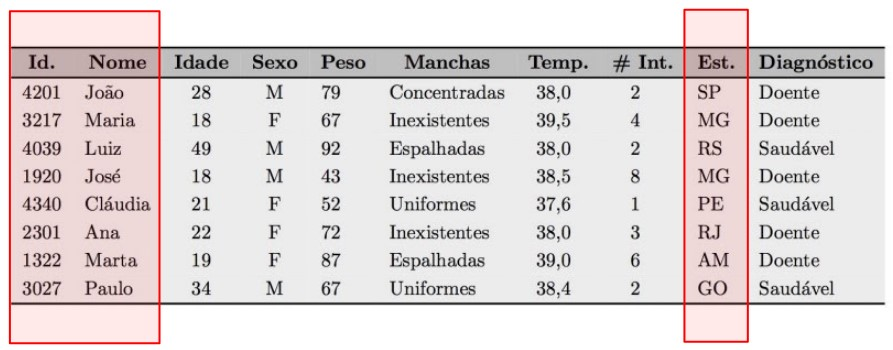
\includegraphics[scale=0.5]{Figuras/slide02_01.jpg}
\end{figure}

\end{ftst}

%=====

\begin{ftst}{Amostragem}{Pré-processamento de dados}
\justifying
A amostragem é um processo usado na análise estatística em que um número predeterminado de observações é obtido de uma população maior.
\vone
Algoritmos de aprendizagem de máquina podem ter dificuldade em lidar com um número grande de objetos.
\vone
Eficiência computacional X acurácia (taxa de predições corretas).
\vone
Muitas vezes, o uso de uma amostra leva ao mesmo desempenho obtido com o uso do conjunto completo, porém com um custo computacional muito menor.

\end{ftst}

%=====

\begin{ftst}{Amostragem}{Pré-processamento de dados}
\justifying
Deve ser observado que uma amostra pequena pode não representar bem o problema que se deseja modelar.
\vone
A amostra deve ser representativa do conjunto de dados original.

\begin{figure}
    \centering
    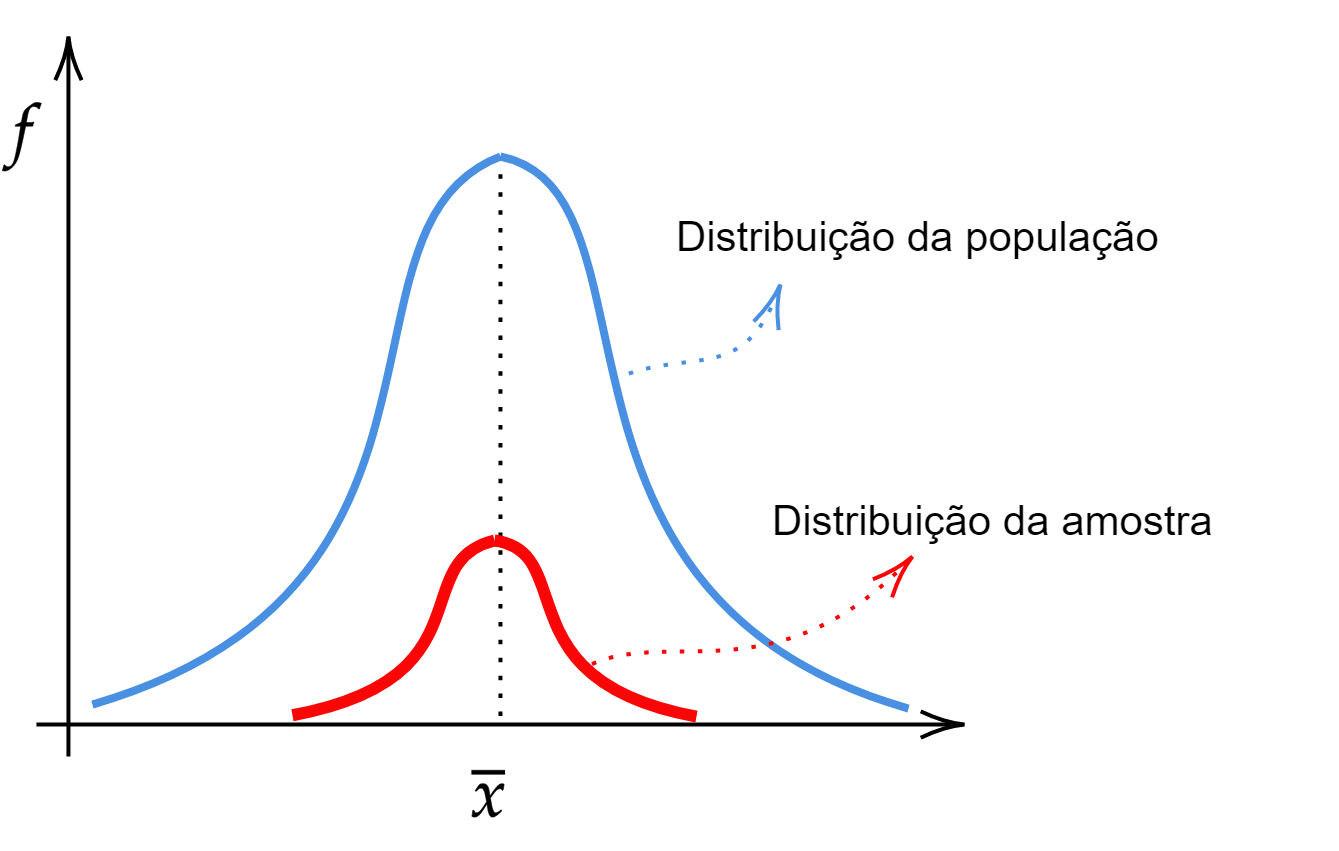
\includegraphics[scale=0.17]{Figuras/slide02_02.png}
\end{figure}

\end{ftst}

%=====

\begin{ftst}{Amostragem}{Pré-processamento de dados}
\justifying
\textbf{Técnicas de amostragem:}
\vone
\begin{itemize}
    \item Amostragem aleatória simples.
    \vone
    \item Amostragem estratificada: usada em problemas de classificação.
    - Manter o mesmo número de objetos em ambas as classes.
    
    - Manter a proporção do número de objetos do conjunto original.
    \vone
    \item Amostragem progressiva: começa com uma amostra pequena e aumenta progressivamente enquanto a acurácia continuar a melhorar.
\end{itemize}

\end{ftst}

%=====

\begin{ftst}{Dados desbalanceados}{Pré-processamento de dados}
\justifying
O problema de \textbf{dados desbalanceados} é tópico da área de classificação de dados.
\vone
Esse problema é comum em aplicações em que dados de um subconjunto das classes aparecem com uma frequência maior que os dados das demais classes.
\vone
Exemplo: supondo que 80\% dos pacientes que vão a um determinado hospital estão doentes, seu conjunto de dados apresentará então 20\% de seus objetos relacionados a pacientes saudáveis.
\vone
\textit{Classe majoritária:} pacientes doentes.

\textit{Classe minoritária:} pacientes saudáveis.

\end{ftst}

%=====

\begin{ftst}{Dados desbalanceados}{Pré-processamento de dados}
\justifying
Quando algoritmos são alimentados com dados desbalanceados, eles tendem a favorecer a classificação de novos dados na classe majoritária.
\vone
Caso o balanceamento das classes não seja possível, o balanceamento artificial, através da criação de \textbf{amostras sintéticas}, pode ser usado.
\vone

\end{ftst}

%=====

\begin{ftst}{Limpeza de dados}{Pré-processamento de dados}
\justifying
Conjuntos de dados podem apresentar dificuldades relacionadas à qualidade dos dados:
\begin{itemize}
    \item dados ruidosos: que possuem erros ou valores discrepantes.
    \item inconsistentes: que contradizem valores de outros atributos do mesmo objeto.
    \item redundantes: dois ou mais objetos com mesmos valores em todos os atributos.
    \item incompletos: ausência de valores.
\end{itemize}
\vone
Essas deficiências podem ser causadas por: problemas em equipamentos que realizam coleta, transmissão e armazenamento dos dados ou por erro humano.

\end{ftst}

%=====

\begin{ftst}{Limpeza de dados}{Pré-processamento de dados}
\justifying
Dados incompletos:
\small
\begin{itemize}
    \item Eliminar o objeto com valores ausentes.
    \item Utilizar média, moda ou mediana dos valores conhecidos do atributo.
    
    - Ex: usar a média do atributo de uma classe.
    
    - Ex: para dados que possuem relação temporal, a medida pode ser calculada usando os objetos associados ao instante imediatamente anterior e posterior ao objeto modificado.
    \item usar um modelo para estimar o valor do atributo.
\end{itemize}
\vone
\normalsize
Dados inconsistentes e redundantes:
\begin{itemize}
    \item Exclusão.
\end{itemize}
\vone
Ruídos podem ser dados inconsistentes ou \textit{outliers}!
\end{ftst}

%=====

\begin{ftst}{Transformação nos dados}{Pré-processamento de dados}
\justifying
\textbf{Conversão Simbólico-Numérico}
\vone
Quando o atributo é nominal e assume apenas dois valores, se denotam a presença ou ausência de uma característica ou se apresentam uma relação de ordem, um dígito binário é suficiente.
\vone
Exemplo: (doente = 0 | saudável = 1) ou (frio = 0 | quente = 1).




\end{ftst}

%=====

\begin{ftst}{Transformação nos dados}{Pré-processamento de dados}
\justifying
\textbf{Conversão Simbólico-Numérico}
\vone
Para atributos com mais de dois valores:
\vone
\begin{itemize}
    \item Se não houver uma relação de ordem, a inexistência também dever continuar após a transformação.
    \item Se existe a relação de ordem, a codificação deve preservá-la.
\end{itemize}

\begin{figure}
    \centering
    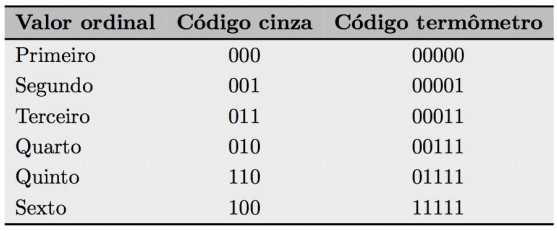
\includegraphics[scale=0.6]{Figuras/slide02_03.jpg}
\end{figure}

\end{ftst}

%=====

\begin{ftst}{Transformação nos dados}{Pré-processamento de dados}
\justifying
\textbf{Conversão Numérico-Simbólico}
\vone

\begin{itemize}
    \item Se o atributo for do tipo discreto e binário, com apenas dois valores, basta associar um nome a cada valor.
    \item Se o atributo for formado por uma sequência de bits sem uma relação de ordem, cada sequência pode ser substituída por um nome.
    \item Nos demais casos, usar um método de discretização que melhor represente o domínio do problema.
\end{itemize}

\end{ftst}

%=====

\begin{ftst}{Transformação nos dados}{Pré-processamento de dados}
\justifying
\textbf{Atributos numéricos:} algumas vezes um atributo numérico precisa ser transformado em outro valor numérico. Isso ocorre quando:
\vone

\begin{itemize}
    \item Os limites inferior e superior de valores dos atributos são muito diferentes.
    \item Vários atributos estão em escalas diferentes.
\end{itemize}
\vone
Essa transformação é realizada para evitar que um atributo predomine sobre o outro.

\end{ftst}

%=====

\begin{ftst}{Transformação nos dados}{Pré-processamento de dados}
\justifying
\textbf{Normalização por reescala:} defini uma nova escala de valores, limite mínimo e máximo, para todos os atributos.
\vone
Exemplo de normalização min-max:
\begin{equation}
    v_{novo} = min + \frac{v_{atual}- menor}{maior - menor}(max-min)
\end{equation}
\vone
\textbf{*}Para limite superior 1 e inferior 0, max = 1 e min = 0.

\end{ftst}

%=====

\begin{ftst}{Transformação nos dados}{Pré-processamento de dados}
\justifying
\textbf{Normalização por padronização:} defini um valor central e um valor de espalhamento comuns para todos os atributos.
\vone
Exemplo de padronização dos valores com média ($\mu$) = 0 e variância ($\sigma$) = 1:

\begin{equation}
    v_{novo} = \frac{v_{atual}- \mu}{maior - \sigma}
\end{equation}


\end{ftst}

%=====

\begin{ftst}{Redução de dimensionalidade}{Pré-processamento de dados}
\justifying
\textbf{Maldição da dimensionalidade:} se cada atributo é visto como uma coordenada em um espaço d-dimensional, em que d é o número de atributos, o hipervolume que representa esse espaço cresce exponencialmente.
\begin{figure}
    \centering
    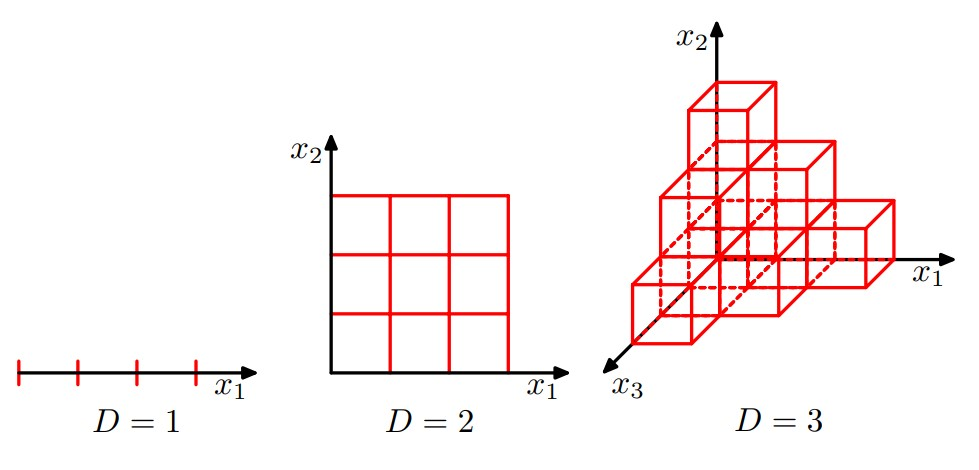
\includegraphics[scale=0.4]{Figuras/slide02_04.jpg}
\end{figure}


\end{ftst}

%=====

\begin{ftst}{Redução de dimensionalidade}{Pré-processamento de dados}
\justifying
Na prática, a maldição da dimensionalidade implica que para um dado tamanho de amostras, existe um número máximo de características a partir do qual o desempenho do classificador irá degradar, ao invés de melhorar.
\begin{figure}
    \centering
    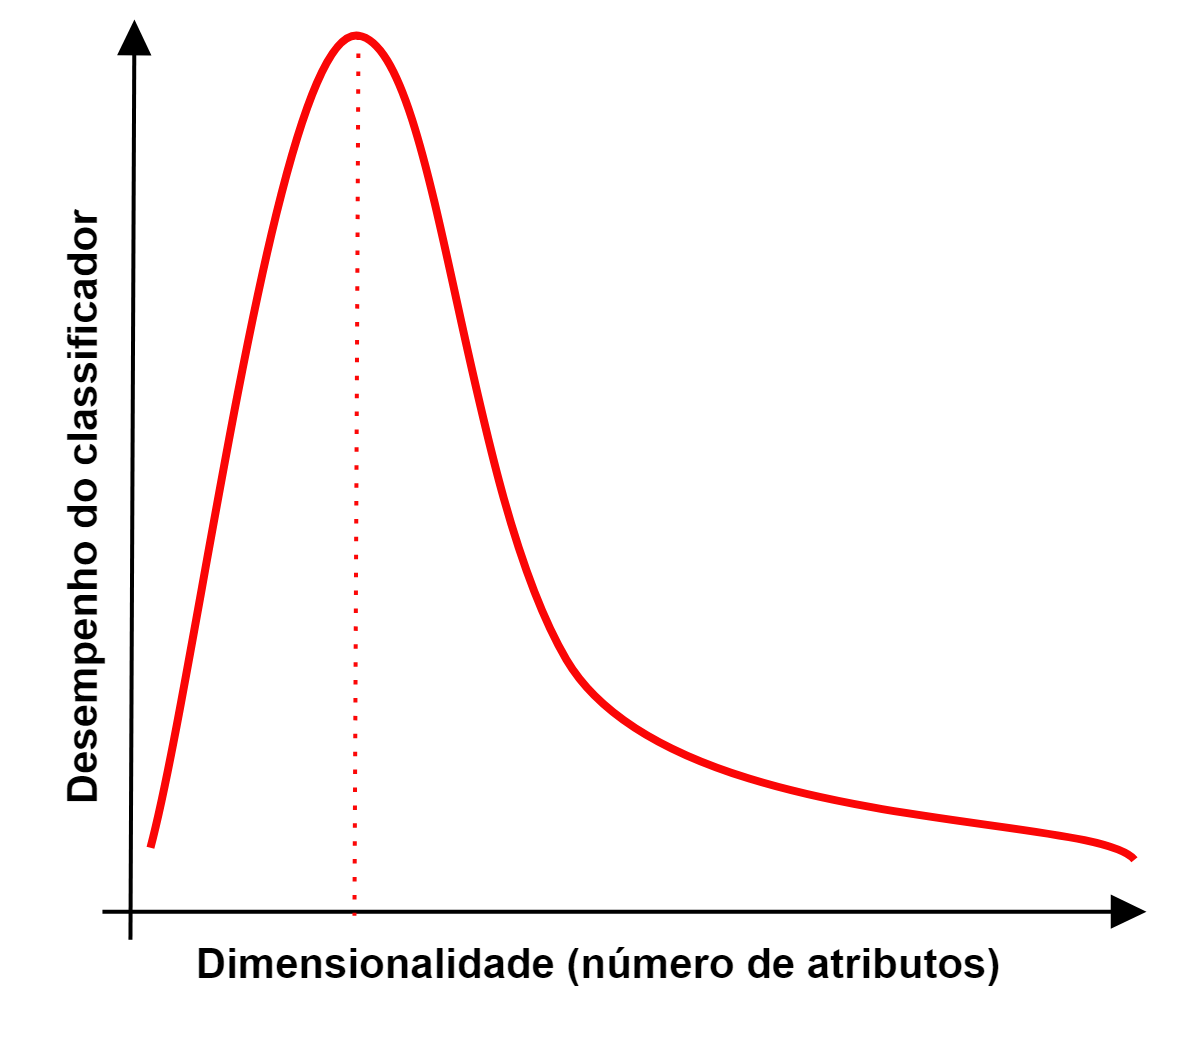
\includegraphics[scale=0.15]{Figuras/slide02_05.png}
\end{figure}


\end{ftst}

%=====

\begin{ftst}{Redução de dimensionalidade}{Pré-processamento de dados}

\textbf{Técnicas de redução de dimensionalidade:}
\small
\vone
\begin{itemize}
 \item \textit{Agregação:} substituem os atributos originais por novos atributos formados pela combinação de grupos de atributos e consequentemente resulta em perda de informação.
    
 - Exemplo: análise de componentes principais (PCA).
\vone
 \item \textit{Seleção:} mantêm uma parte dos atributos originais e descartam os demais atributos. Essas técnicas procuram um subconjunto ótimo de atributos de acordo com um determinado critério.
    
- Exemplo: embutida, baseada em filtro ou baseada em \textit{wrapper}.
\end{itemize}


\end{ftst}

%=====






\end{document}